\documentclass{article}

\usepackage{listings}
\usepackage{graphicx}

\title{Day 1, exercise 4: Vigilance}
\author{Richel Bilderbeek}
\date{\today}

\begin{document}

\maketitle

\begin{abstract}
This article is created within the CAS program Maxima
and shows how to do algebraic manipuations and graphical plotting.
The output is in \LaTeX~ format.
\end{abstract}
\section{Exercise}
First, we write down all equations
(for definitions see table \ref{table:table_definition} on page \pageref{table:table_definition}).
\begin{table}[here]
  \centering
  \begin{tabular}{ | r | l | }
    \hline
    symbol & description \\
    \hline
    $v$ & fraction of foraging time invested in being watchful \\
    $S(v)$ & survival probability \\
    $F(v)$ & foraging efficiency \\
    $W(v)$ & fitness \\
    \hline
  \end{tabular}
  \caption{Definitions}
  \label{table:table_definition}
\end{table}
$$S\left(v\right)=v$$
$$F\left(v\right)=1.0-v^2$$
$$W\left(v\right)=-v^2+v+1.0$$
The fitness function plotted is plotted in figure 
\ref{figure:figure_fitness} on page \pageref{figure:figure_fitness}.\\
\begin{figure}[here]
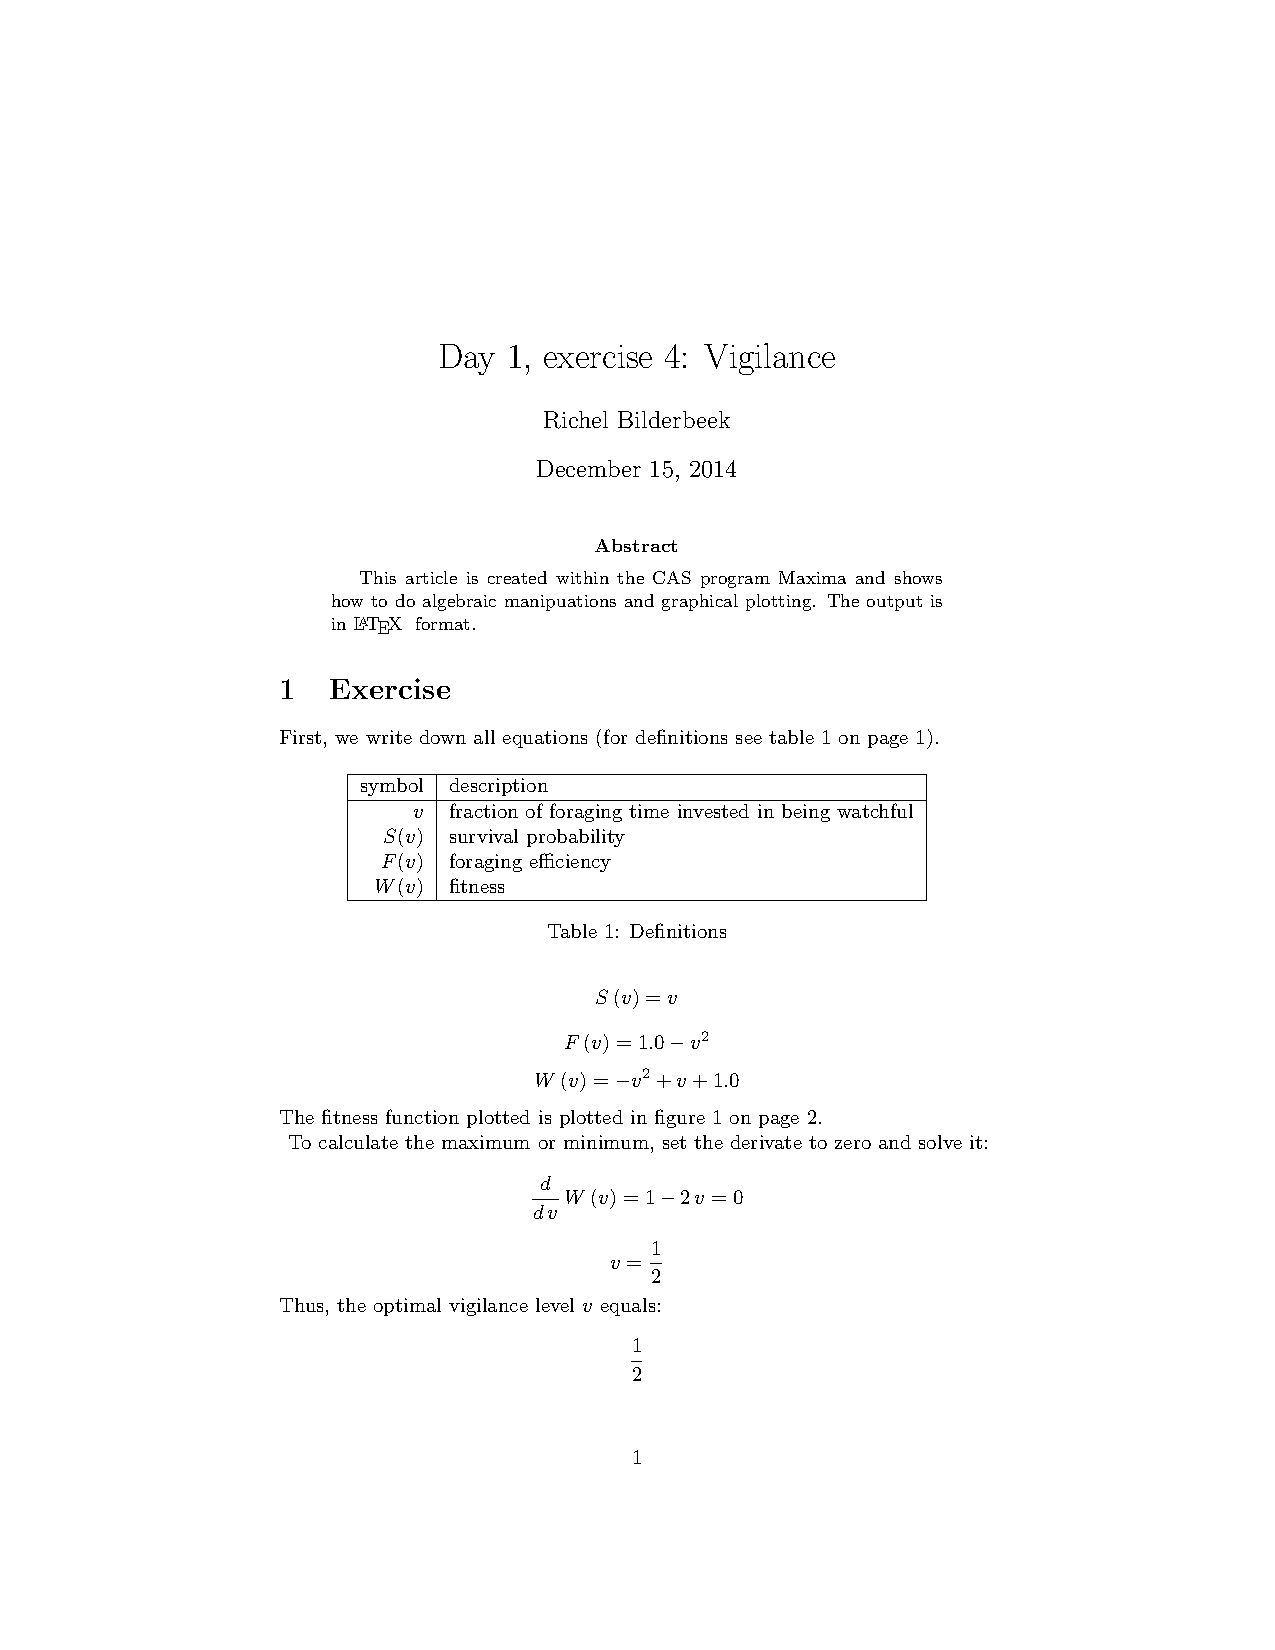
\includegraphics[width=1\textwidth]{/home/richel/GitHubs/Maxima/Day1_4_vigilance_output.pdf}\\\\
  \caption{Fitness function}
  \label{figure:figure_fitness}
\end{figure}
To calculate the maximum or minimum, set the derivate to zero and solve it:
$${{d}\over{d\,v}}\,W\left(v\right)=1-2\,v=0$$
$$v={{1}\over{2}}$$
Thus, the optimal vigilance level $v$ equals:$${{1}\over{2}}$$

This optimal vigilance level results in a fitness of:$$W\left({{1}\over{2}}\right)=1.25$$

To find out if it is a fitness minimum or maximum,
calculate the second derivative
and find out its value at the minimum or maximum:
$${{d^2}\over{d\,v^2}}\,W\left(v\right)=-2$$
Thus, it is a maximum.

\appendix

\section{Script file}

\lstinputlisting[language=C++,showstringspaces=false,breaklines=true,frame=single]{Day1_4_vigilance.sh}

\section{Maxima file}

\lstinputlisting[language=C++,showstringspaces=false,breaklines=true,frame=single]{Day1_4_vigilance.txt}

\section{\LaTeX~file}

\lstinputlisting[language=tex,showstringspaces=false,breaklines=true,frame=single]{Day1_4_vigilance_output.tex}

\end{document}
